%%%%%%%%%%%%%%%%%%%%%%%%%%%%%%%%%%%%%%%%%%%%%%%%%%%%%%%%%%%%%%%%%%%%%%%%%%%%%%%%%%
\begin{frame}[fragile]\frametitle{}
\begin{center}
{\Large RAG Framework}
\end{center}
\end{frame}

%%%%%%%%%%%%%%%%%%%%%%%%%%%%%%%%%%%%%%%%%%%%%%%%%%%%%%%%%%%%%%%%%%%%%%%%%%%%%%%%%%
\begin{frame}[fragile]\frametitle{RAG Framework Basics}
  \begin{itemize}
    \item Three key modules: Retriever, Reranker, Generator
    \item Retrieval flow: identify, score, and generate
    \item External knowledge sources enhance language generation
  \end{itemize}
\end{frame}

%%%%%%%%%%%%%%%%%%%%%%%%%%%%%%%%%%%%%%%%%%%%%%%%%%%%%%%%%%%%%%%%%%%%%%%%%%%%%%%%%%
\begin{frame}[fragile]\frametitle{Innovations in Retriever Models}
  \begin{itemize}
    \item Knowledge Enhanced Dual-Encoders for LLMs
    \item Poly-encoders for efficient SLMs
    \item Term Weighting Optimization using ANCE and ANS
    \item Integration of Semantic Term Matching with Condenser
  \end{itemize}
\end{frame}

%%%%%%%%%%%%%%%%%%%%%%%%%%%%%%%%%%%%%%%%%%%%%%%%%%%%%%%%%%%%%%%%%%%%%%%%%%%%%%%%%%
\begin{frame}[fragile]\frametitle{Reranker Innovations}
  \begin{itemize}
    \item Cross-Encoders and Poly-encoders
    \item Weak Supervision Scaling for efficiency
    \item Specialized Reranker Architectures for accuracy
  \end{itemize}
\end{frame}

%%%%%%%%%%%%%%%%%%%%%%%%%%%%%%%%%%%%%%%%%%%%%%%%%%%%%%%%%%%%%%%%%%%%%%%%%%%%%%%%%%
\begin{frame}[fragile]\frametitle{Innovations in Generator Models}
  \begin{itemize}
    \item Evidence Fusion decisions for LLMs and SLMs
    \item Conditioning Design with working memory for LLMs
    \item Efficiency Optimized Architectures for throughput
  \end{itemize}
\end{frame}

%%%%%%%%%%%%%%%%%%%%%%%%%%%%%%%%%%%%%%%%%%%%%%%%%%%%%%%%%%%%%%%%%%%%%%%%%%%%%%%%%%
\begin{frame}[fragile]\frametitle{Hybrid RAG with Heterogeneous Models}
  \begin{itemize}
    \item Integration of both LLMs and SLMs
    \item Use of larger models for initial retrieval
    \item Specialization of SLMs for specific content forms
  \end{itemize}
\end{frame}

%%%%%%%%%%%%%%%%%%%%%%%%%%%%%%%%%%%%%%%%%%%%%%%%%%%%%%%%%%%%%%%%%%%%%%%%%%%%%%%%%%
\begin{frame}[fragile]\frametitle{Key Takeaways}
  \begin{itemize}
    \item RAG complements language models with external knowledge
    \item Innovations in Retriever, Reranker, and Generator modules
    \item Hybrid RAG systems for optimal balance
  \end{itemize}
\end{frame}


%%%%%%%%%%%%%%%%%%%%%%%%%%%%%%%%%%%%%%%%%%%%%%%%%%%%%%%%%%%%%%%%%%%%%%%%%%%%%%%%%%
\begin{frame}[fragile]\frametitle{RAG Pipeline Considerations}
    \begin{itemize}
        \item RAG expands non-parametric memory of \#llms.
        \item Indexing pipeline creates a knowledge base for the RAG pipeline.
        \item Crucial step: Splitting documents into manageable chunks (Chunking).
            \begin{itemize}
                \item Large chunks are harder to search; chunking aids in better indexing.
                \item Retrieved context should be significantly smaller than the LLM's context window.
            \end{itemize}
        \item Chunking strategies depend on:
            \begin{itemize}
                \item Nature of the content.
                \item Embedding models chosen.
                \item Length/Complexity of user inputs (context window limitations).
                \item Use Case.
            \end{itemize}
    \end{itemize}
\end{frame}


%%%%%%%%%%%%%%%%%%%%%%%%%%%%%%%%%%%%%%%%%%%%%%%%%%%%%%%%%%%
\begin{frame}[fragile]\frametitle{RAG Pipeline}

	\begin{center}
	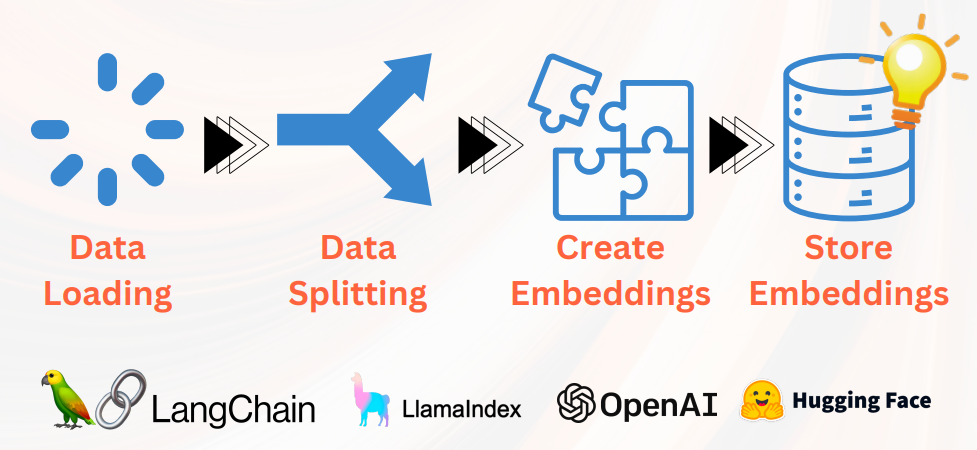
\includegraphics[width=\linewidth,keepaspectratio]{rag15}
	\end{center}

	{\tiny (Ref: Knowledge Brain RAG - Abhinav  Kimothi)}

\end{frame}




%%%%%%%%%%%%%%%%%%%%%%%%%%%%%%%%%%%%%%%%%%%%%%%%%%%%%%%%%%%%%%%%%%%%%%%%%%%%%%%%%%
\begin{frame}[fragile]{Loading Data}
    \begin{itemize}
        \item Websites \& HTML pages
        \item Documents like word, pdf etc.
        \item Code in python, java etc.
        \item Data in json, csv etc.
        \item APIs
        \item File Directories
        \item Databases
        \item And many more
    \end{itemize}
\end{frame}

%%%%%%%%%%%%%%%%%%%%%%%%%%%%%%%%%%%%%%%%%%%%%%%%%%%%%%%%%%%%%%%%%%%%%%%%%%%%%%%%%%
\begin{frame}[fragile]{Document Splitting}
    \begin{itemize}
        \item Websites \& HTML pages
        \item Documents like word, pdf etc.
        \item Code in python, java etc.
        \item Data in json, csv etc.
        \item APIs
        \item File Directories
        \item Databases
        \item And many more
    \end{itemize}
\end{frame}


%%%%%%%%%%%%%%%%%%%%%%%%%%%%%%%%%%%%%%%%%%%%%%%%%%%%%%%%%%%%%%%%%%%%%%%%%%%%%%%%%%
\begin{frame}[fragile]{RAG Pipeline Considerations}
    \begin{itemize}
        \item RAG expands non-parametric memory of \#llms.
        \item Indexing pipeline creates a knowledge base for the RAG pipeline.
        \item Crucial step: Splitting documents into manageable chunks (Chunking).
            \begin{itemize}
                \item Large chunks are harder to search; chunking aids in better indexing.
                \item Retrieved context should be significantly smaller than the LLM's context window.
            \end{itemize}
        \item Chunking strategies depend on:
            \begin{itemize}
                \item Nature of the content.
                \item Embedding models chosen.
                \item Length/Complexity of user inputs (context window limitations).
                \item Use Case.
            \end{itemize}
    \end{itemize}
\end{frame}

%%%%%%%%%%%%%%%%%%%%%%%%%%%%%%%%%%%%%%%%%%%%%%%%%%%%%%%%%%%%%%%%%%%%%%%%%%%%%%%%%%
\begin{frame}[fragile]{Importance of Document Chunking}
  \begin{itemize}
    \item \textbf{Ease of Search:} Larger data chunks are harder to search efficiently, making document splitting crucial for better indexation.
    \item \textbf{Context Window Size:} Large Language Models (LLMs) have finite token limits, necessitating document chunking to fit within the context window.
  \end{itemize}
\end{frame}

%%%%%%%%%%%%%%%%%%%%%%%%%%%%%%%%%%%%%%%%%%%%%%%%%%%%%%%%%%%%%%%%%%%%%%%%%%%%%%%%%%
\begin{frame}[fragile]{Considerations for Chunking Strategies}
  \begin{itemize}
    \item \textbf{Nature of Content:} Adapt chunking strategy based on document length (articles vs. tweets) and the chosen model.
    \item \textbf{Embedding Model:} Choice of embedding model influences the optimal chunking strategy based on performance with specific lengths.
    \item \textbf{User Queries:} Adjust chunking based on expected query length and complexity for improved correlation.
    \item \textbf{Application-Specific Requirements:} Tailor chunking to application needs, considering token limits of downstream models.
  \end{itemize}
\end{frame}

%%%%%%%%%%%%%%%%%%%%%%%%%%%%%%%%%%%%%%%%%%%%%%%%%%%%%%%%%%%%%%%%%%%%%%%%%%%%%%%%%%
\begin{frame}[fragile]{Chunking Methods Overview}
  \begin{itemize}
    \item \textbf{Divide and Merge Approach:} Split text into meaningful units (sentences), merge into larger chunks, and treat them as independent segments.
    \item \textbf{Pre-determined Size and Overlap:} Determine chunk size and specify overlap to maintain contextual continuity between chunks.
  \end{itemize}
\end{frame}

%%%%%%%%%%%%%%%%%%%%%%%%%%%%%%%%%%%%%%%%%%%%%%%%%%%%%%%%%%%%%%%%%%%%%%%%%%%%%%%%%%
\begin{frame}[fragile]{Text Splitting Approaches}
  \begin{itemize}
    \item \textbf{Split by Character:} Divide text based on characters, measuring chunk size by the number of characters.
    \item \textbf{Recursive Split by Character:} Hierarchical splitting using a list of characters for gradual chunking, recommended for generic text.
    \item \textbf{Split by Tokens:} Utilize token limits of LLMs, count tokens while creating chunks, and leverage tokenizers (e.g., Hugging Face Tokenizer).
  \end{itemize}
\end{frame}

%%%%%%%%%%%%%%%%%%%%%%%%%%%%%%%%%%%%%%%%%%%%%%%%%%%%%%%%%%%%%%%%%%%%%%%%%%%%%%%%%%
\begin{frame}[fragile]{Hugging Face Tokenizer}
  \begin{itemize}
    \item \textbf{Tokenization Platform:} Hugging Face is a widely used platform for LLMs, providing access to models along with their tokenizers.
  \end{itemize}
\end{frame}

%%%%%%%%%%%%%%%%%%%%%%%%%%%%%%%%%%%%%%%%%%%%%%%%%%%%%%%%%%%%%%%%%%%%%%%%%%%%%%%%%%
\begin{frame}[fragile]{Specialized Chunking}
  \begin{itemize}
    \item \textbf{Document Structure Honoring:} Consider specific document structures (HTML, Markdown, Latex, code) for preserving context during chunking.
  \end{itemize}
\end{frame}

%%%%%%%%%%%%%%%%%%%%%%%%%%%%%%%%%%%%%%%%%%%%%%%%%%%%%%%%%%%%%%%%%%%%%%%%%%%%%%%%%%
\begin{frame}[fragile]{Things to Keep in Mind}
  \begin{itemize}
    \item \textbf{Data Quality:} Preprocess data for optimal chunk size, removing noise elements like HTML tags.
    \item \textbf{Balance Context and Accuracy:} Find a balance between preserving context and maintaining accuracy in chunking.
    \item \textbf{Test Different Chunk Sizes:} Evaluate and compare performance by creating embeddings for different chunk sizes in the index through queries.
  \end{itemize}
\end{frame}

%%%%%%%%%%%%%%%%%%%%%%%%%%%%%%%%%%%%%%%%%%%%%%%%%%%%%%%%%%%%%%%%%%%%%%%%%%%%%%%%%%
\begin{frame}[fragile]{Embeddings}
  \begin{itemize}
    \item All ML/AI models operate with numerical data.
    \item Embeddings are n-dimensional matrices capturing meaningful relationships in data.
    \item Word embeddings represent words as vectors, a crucial concept for RAG applications.
  \end{itemize}
\end{frame}

%%%%%%%%%%%%%%%%%%%%%%%%%%%%%%%%%%%%%%%%%%%%%%%%%%%%%%%%%%%%%%%%%%%%%%%%%%%%%%%%%%
\begin{frame}[fragile]{Generalization through Transfer Learning}
  \begin{itemize}
    \item Embeddings enable transfer learning, allowing generalization across tasks and domains.
    \item Transfer learning facilitates switching contexts seamlessly.
    \item Popularity of embeddings in ML applications is attributed to this generalization capability.
  \end{itemize}
\end{frame}

%%%%%%%%%%%%%%%%%%%%%%%%%%%%%%%%%%%%%%%%%%%%%%%%%%%%%%%%%%%%%%%%%%%%%%%%%%%%%%%%%%
\begin{frame}[fragile]{Popular Embedding Models}
  \begin{columns}
    \column{0.5\textwidth}
      \begin{itemize}
        \item \textbf{word2vec:}
          \begin{itemize}
            \item Pre-trained word embeddings by Google.
            \item Vector representation of words.
          \end{itemize}
        \item \textbf{GLOVE:}
          \begin{itemize}
            \item Global Vectors model capturing statistics at a global level.
          \end{itemize}
      \end{itemize}
    \column{0.5\textwidth}
      \begin{itemize}
        \item \textbf{fastText:}
          \begin{itemize}
            \item Embeddings built from characters instead of words.
            \item Developed by Facebook's AI research.
          \end{itemize}
        \item \textbf{Elmo:}
          \begin{itemize}
            \item Embeddings from Language Models based on bidirectional LSTM.
          \end{itemize}
        \item \textbf{BERT:}
          \begin{itemize}
            \item Bidirectional Encoder Representations from Transformers.
            \item Transformer-based approach.
          \end{itemize}
      \end{itemize}
  \end{columns}
\end{frame}

%%%%%%%%%%%%%%%%%%%%%%%%%%%%%%%%%%%%%%%%%%%%%%%%%%%%%%%%%%%%%%%%%%%%%%%%%%%%%%%%%%
\begin{frame}[fragile]{Choosing Embeddings}
  \begin{itemize}
    \item \textbf{Landscape Overview:}
      \begin{itemize}
        \item The release of ChatGPT and the LLM Wars increased the development of embedding models.
        \item Evolving standards for evaluating LLMs and embeddings.
      \end{itemize}
    \item \textbf{Use Case Variability:}
      \begin{itemize}
        \item No universal answer to "Which embeddings model to use?"
        \item Some embeddings may perform better for specific use cases (summarization, text generation, classification).
      \end{itemize}
  \end{itemize}
\end{frame}

%%%%%%%%%%%%%%%%%%%%%%%%%%%%%%%%%%%%%%%%%%%%%%%%%%%%%%%%%%%%%%%%%%%%%%%%%%%%%%%%%%
\begin{frame}[fragile]{MTEB Leaderboard}
  \begin{itemize}
    \item \textbf{Hugging Face's MTEB Leaderboard:}
      \begin{itemize}
        \item Evaluates various embedding models across seven use cases.
        \item Use cases include Classification, Clustering, Pair Classification, Reranking, Retrieval, Semantic Textual Similarity (STS), and Summarization.
      \end{itemize}
  \end{itemize}
\end{frame}

%%%%%%%%%%%%%%%%%%%%%%%%%%%%%%%%%%%%%%%%%%%%%%%%%%%%%%%%%%%%%%%%%%%%%%%%%%%%%%%%%%
\begin{frame}[fragile]{Cost Considerations}
  \begin{itemize}
    \item \textbf{OpenAI Models:}
      \begin{itemize}
        \item Significant costs with OpenAI models, especially with large document sets.
        \item Costs depend on the implementation for open-source models.
      \end{itemize}
  \end{itemize}
\end{frame}

%%%%%%%%%%%%%%%%%%%%%%%%%%%%%%%%%%%%%%%%%%%%%%%%%%%%%%%%%%%%%%%%%%%%%%%%%%%%%%%%%%
\begin{frame}[fragile]{Creating Embeddings}
  \begin{itemize}
    \item \textbf{Embedding Creation:}
      \begin{itemize}
        \item After choosing an embedding model, various methods exist for creating embeddings.
        \item Tools like LlamaIndex and LangChain assist in converting documents into vector embeddings.
        \item Directly use services from providers or obtain embeddings from HuggingFace.
      \end{itemize}
  \end{itemize}
\end{frame}

%%%%%%%%%%%%%%%%%%%%%%%%%%%%%%%%%%%%%%%%%%%%%%%%%%%%%%%%%%%%%%%%%%%%%%%%%%%%%%%%%%
\begin{frame}[fragile]{Conclusion}
  \begin{itemize}
    \item Embeddings are essential for RAG applications.
    \item The choice of embeddings depends on use cases, and no one-size-fits-all solution exists.
    \item Continuous evolution in the landscape necessitates staying updated with emerging models and standards.
  \end{itemize}
\end{frame}

%%%%%%%%%%%%%%%%%%%%%%%%%%%%%%%%%%%%%%%%%%%%%%%%%%%%%%%%%%%%%%%%%%%%%%%%%%%%%%%%%%
\begin{frame}[fragile]{Vector Databases}
  \begin{itemize}
    \item Last step in the indexing pipeline is storage.
    \item Vector Database - specialized database for indexing and storing embeddings.
    \item Vector Index (e.g., FAISS) enhances search and retrieval of vector embeddings.
    \item Vector Databases include features like data management, metadata storage, scalability, integrations, security, etc.
  \end{itemize}
\end{frame}

%%%%%%%%%%%%%%%%%%%%%%%%%%%%%%%%%%%%%%%%%%%%%%%%%%%%%%%%%%%%%%%%%%%%%%%%%%%%%%%%%%
\begin{frame}[fragile]{Popular Vector Databases}
  \begin{itemize}
    \item FAISS: Facebook AI Similarity Search (2017)
    \item Pinecone: Managed Vector DB for large scale
    \item Weaviate: Open source vector database for objects and vectors
    \item Chroma: Open source vector database
  \end{itemize}
\end{frame}

%%%%%%%%%%%%%%%%%%%%%%%%%%%%%%%%%%%%%%%%%%%%%%%%%%%%%%%%%%%%%%%%%%%%%%%%%%%%%%%%%%
\begin{frame}[fragile]{Anticipated Growth in Vector Storage}
  \begin{itemize}
    \item Major database players likely to add vector indexing capabilities.
    \item Growing demand for vector storage across industries.
  \end{itemize}
\end{frame}

%%%%%%%%%%%%%%%%%%%%%%%%%%%%%%%%%%%%%%%%%%%%%%%%%%%%%%%%%%%%%%%%%%%%%%%%%%%%%%%%%%
\begin{frame}[fragile]{Choosing a Vector Database}
  \begin{itemize}
    \item Consider nuances of use case matching with database's value proposition.
    \item Balance search accuracy and query speed based on application needs.
    \item Weigh flexibility vs potential performance impacts.
    \item Evaluate data durability vs fast query performance.
    \item Assess tradeoffs between local storage and cloud storage benefits.
    \item Consider integration control via libraries vs ease-of-use through APIs.
    \item Compare algorithm optimizations, query features, indexing complexity.
  \end{itemize}
\end{frame}

%%%%%%%%%%%%%%%%%%%%%%%%%%%%%%%%%%%%%%%%%%%%%%%%%%%%%%%%%%%%%%%%%%%%%%%%%%%%%%%%%%
\begin{frame}[fragile]{Storing Embeddings in Vector DBs}
  \begin{itemize}
    \item For quick prototyping: LangChain and LlamaIndex.
    \item Implementation depends on DB choice, use case, and volume.
    \item Example with FAISS from \texttt{langchain.vectorstores}:
      \begin{itemize}
        \item Loading text file with TextLoader.
        \item Splitting text into chunks with RecursiveCharacterTextSplitter.
        \item Creating embeddings using OpenAIEmbeddings.
        \item Storing embeddings into FAISS vector index.
      \end{itemize}
  \end{itemize}
\end{frame}

%%%%%%%%%%%%%%%%%%%%%%%%%%%%%%%%%%%%%%%%%%%%%%%%%%%%%%%%%%%%%%%%%%%%%%%%%%%%%%%%%%
\begin{frame}[fragile]\frametitle{}
\begin{center}
{\Large Retrieval for RAG}
\end{center}
\end{frame}

%%%%%%%%%%%%%%%%%%%%%%%%%%%%%%%%%%%%%%%%%%%%%%%%%%%%%%%%%%%%%%%%%%%%%%%%%%%%%%%%%%
\begin{frame}[fragile]\frametitle{Retrieval in RAG Value Chain}
\begin{itemize}
    \item Critical step: Searching and retrieving relevant information (documents).
    \item Retriever is responsible for fetching correct information for user queries.
\end{itemize}
\end{frame}

%%%%%%%%%%%%%%%%%%%%%%%%%%%%%%%%%%%%%%%%%%%%%%%%%%%%%%%%%%%
\begin{frame}[fragile]\frametitle{RAG Retrieval}


		\begin{center}
		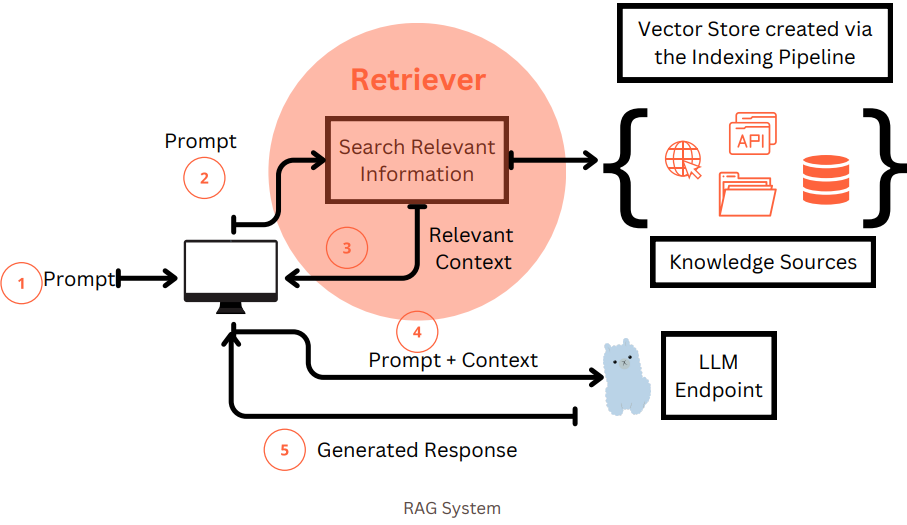
\includegraphics[width=\linewidth,keepaspectratio]{rag23}
		\end{center}

{\tiny (Ref: Knowledge Brain RAG - Abhinav  Kimothi)}

\end{frame}


%%%%%%%%%%%%%%%%%%%%%%%%%%%%%%%%%%%%%%%%%%%%%%%%%%%%%%%%%%%%%%%%%%%%%%%%%%%%%%%%%%
\begin{frame}[fragile]\frametitle{Popular Retrieval Methods}
\begin{itemize}
    \item \textbf{Similarity Search:} Uses vector databases for backbone. Calculates similarity by vector distance.
    \item \textbf{Maximum Marginal Relevance (MMR):} Addresses redundancy, considers relevance in terms of new information.
    \item \textbf{Multi-query Retrieval:} Automates prompt tuning, generates diverse queries, combines results for a comprehensive set.
    \item \textbf{Contextual Compression:} Squeezes down long documents to important parts matching the search.
    \item \textbf{Multi Vector Retrieval:} Stores more than one vector in a document for efficient matching.
\end{itemize}
\end{frame}

%%%%%%%%%%%%%%%%%%%%%%%%%%%%%%%%%%%%%%%%%%%%%%%%%%%%%%%%%%%%%%%%%%%%%%%%%%%%%%%%%%
\begin{frame}[fragile]\frametitle{Additional Retrieval Methods}
\begin{itemize}
    \item \textbf{Parent Document Retrieval:} Self-querying retriever turns natural language questions into structured queries for efficient and accurate search.
    \item \textbf{Time-weighted Retrieval:} Supplements semantic similarity search with time delay, giving more weight to fresher or more used documents.
    \item \textbf{Ensemble Techniques:} Multiple methods used together, structure defined by use cases.
\end{itemize}
\end{frame}

%%%%%%%%%%%%%%%%%%%%%%%%%%%%%%%%%%%%%%%%%%%%%%%%%%%%%%%%%%%%%%%%%%%%%%%%%%%%%%%%%%
\begin{frame}[fragile]\frametitle{Example: Similarity Search using LangChain}
\begin{itemize}
    \item Loading text file using \texttt{TextLoader}.
    \item Splitting text into chunks using \texttt{RecursiveCharacterTextSplitter}.
    \item Creating embeddings using \texttt{all-MiniLM-L6-v2}.
    \item Storing embeddings into \texttt{Chromadb}.
    \item Retrieving chunks using \texttt{similarity\_search}.
\end{itemize}
\end{frame}

%%%%%%%%%%%%%%%%%%%%%%%%%%%%%%%%%%%%%%%%%%%%%%%%%%%%%%%%%%%%%%%%%%%%%%%%%%%%%%%%%%
\begin{frame}[fragile]\frametitle{}
\begin{center}
{\Large RAG Evaluation}
\end{center}
\end{frame}

%%%%%%%%%%%%%%%%%%%%%%%%%%%%%%%%%%%%%%%%%%%%%%%%%%%%%%%%%%%%%%%%%%%%%%%%%%%%%%%%%%
\begin{frame}[fragile]
\frametitle{Introduction}
\begin{itemize}
    \item Building a PoC RAG pipeline with langchain and llamaindex.
    \item Achieving impressive LLM applications through brief training.
    \item Thorough testing on a production-mirroring dataset is crucial for robustness.
\end{itemize}
\end{frame}

%%%%%%%%%%%%%%%%%%%%%%%%%%%%%%%%%%%%%%%%%%%%%%%%%%%%%%%%%%%%%%%%%%%%%%%%%%%%%%%%%%
\begin{frame}[fragile]
\frametitle{Evaluation Focus}
\begin{itemize}
    \item \textbf{Search \& Retrieval}
    \begin{itemize}
        \item How good is the retrieval of context from the Vector Database?
        \item Relevance to the query.
        \item Presence of noise (irrelevant information).
    \end{itemize}
    \item \textbf{Generation}
    \begin{itemize}
        \item Quality of the generated response.
        \item Grounding in the provided context.
        \item Relevance to the query.
    \end{itemize}
\end{itemize}
\end{frame}

%%%%%%%%%%%%%%%%%%%%%%%%%%%%%%%%%%%%%%%%%%%%%%%%%%%%%%%%%%%%%%%%%%%%%%%%%%%%%%%%%%
\begin{frame}[fragile]
\frametitle{Ragas Framework (2023)}
\begin{itemize}
    \item Developed by Jithin James and Shahul ES.
    \item A state-of-the-art framework for RAG pipeline evaluation.
\end{itemize}
\end{frame}

%%%%%%%%%%%%%%%%%%%%%%%%%%%%%%%%%%%%%%%%%%%%%%%%%%%%%%%%%%%%%%%%%%%%%%%%%%%%%%%%%%
\begin{frame}[fragile]
\frametitle{Evaluation Data}
\begin{itemize}
    \item Set of Queries or Prompts.
    \item Corresponding Response from LLM.
    \item Retrieved Context for each prompt.
    \item Ground Truth or known correct response.
\end{itemize}
\end{frame}

%%%%%%%%%%%%%%%%%%%%%%%%%%%%%%%%%%%%%%%%%%%%%%%%%%%%%%%%%%%%%%%%%%%%%%%%%%%%%%%%%%
\begin{frame}[fragile]
\frametitle{Ragas Metrics: Faithfulness}
\begin{itemize}
    \item Faithfulness $= \frac{\text{Number of generated claims present}}{\text{Total number of claims made in the response}}$
    \item Score Range: (0, 1), higher is better.
\end{itemize}
\end{frame}

%%%%%%%%%%%%%%%%%%%%%%%%%%%%%%%%%%%%%%%%%%%%%%%%%%%%%%%%%%%%%%%%%%%%%%%%%%%%%%%%%%
\begin{frame}[fragile]
\frametitle{Ragas Metrics: Answer Relevancy}
\begin{itemize}
    \item Answer Relevance $= \text{Avg}(\text{Cosine Similarity}(\text{Initial Query, LLM generated Query}[i]))$
    \item Score Range: (0, 1), higher is better.
\end{itemize}
\end{frame}

%%%%%%%%%%%%%%%%%%%%%%%%%%%%%%%%%%%%%%%%%%%%%%%%%%%%%%%%%%%%%%%%%%%%%%%%%%%%%%%%%%
\begin{frame}[fragile]
\frametitle{Ragas Metrics: Context Recall}
\begin{itemize}
    \item Context Relevance $= \frac{\text{Number of Ground Truth sentences in the context}}{\text{Total number of sentences in the Ground Truth}}$
    \item Score Range: (0, 1), higher is better.
\end{itemize}
\end{frame}

%%%%%%%%%%%%%%%%%%%%%%%%%%%%%%%%%%%%%%%%%%%%%%%%%%%%%%%%%%%%%%%%%%%%%%%%%%%%%%%%%%
\begin{frame}[fragile]
\frametitle{Ragas Metrics: Context Precision}
\begin{itemize}
    \item Context Precision @ k $= \frac{\text{Sum(Precision@k)}}{\text{Total number of relevant documents in the top results}}$
    \item Precision @ k $= \frac{\text{True Positives@k}}{\text{True Positives@k + False Positives@k}}$
    \item Score Range: (0, 1), higher is better.
\end{itemize}
\end{frame}

%%%%%%%%%%%%%%%%%%%%%%%%%%%%%%%%%%%%%%%%%%%%%%%%%%%%%%%%%%%%%%%%%%%%%%%%%%%%%%%%%%
\begin{frame}[fragile]
\frametitle{Ragas Metrics: Context Relevancy}
\begin{itemize}
    \item Context Relevance $= \frac{\text{Number of relevant sentences from the context}}{\text{Total number of sentences in the retrieved context}}$
    \item Score Range: (0, 1), higher is better.
\end{itemize}
\end{frame}

%%%%%%%%%%%%%%%%%%%%%%%%%%%%%%%%%%%%%%%%%%%%%%%%%%%%%%%%%%%%%%%%%%%%%%%%%%%%%%%%%%
\begin{frame}[fragile]
\frametitle{Ragas Metrics: Answer Semantic Similarity}
\begin{itemize}
    \item Answer Semantic Similarity $= \text{Similarity}(\text{Generated Response, Ground Truth Response})$
    \item Score Range: (0, 1), higher is better.
\end{itemize}
\end{frame}

%%%%%%%%%%%%%%%%%%%%%%%%%%%%%%%%%%%%%%%%%%%%%%%%%%%%%%%%%%%%%%%%%%%%%%%%%%%%%%%%%%
\begin{frame}[fragile]
\frametitle{Ragas Metrics: Answer Correctness}
\begin{itemize}
    \item Answer Correctness $= \text{Semantic and Factual Similarity between generated response and ground truth response}$
    \item Score Range: (0, 1), higher is better.
\end{itemize}
\end{frame}